\documentclass[12pt]{article}
\usepackage{amsmath}
\usepackage{amssymb}
\usepackage{graphicx}
\usepackage{color}
\usepackage{float}
\begin{document}	
	\title{Simulation framework for chromatin architecture post UV-C irradiation}
\maketitle
\section{The simulation framework}
	We follow \textit{in silico} the dynamics of DNA and nucleosome signal loss from a circular region of interest (ROI) up to 15 minutes post UV-C irradiation followed by a period post repair. To examine the re-organization of the chromatin post UV-C, we compare between the polymer configuration before UV-C and at the end of repair stage. Simulations are performed for a range of UV-C dosage $u$.  
	
	To representing the dynamics of the chromatin in the UV damage micro-environment, simulations are performed in a three-dimensional spherical domain with reflecting boundaries. Results are reported as the projected values on the x-y plane, in-line with the maximal Z-projection reported experimentally \cite{adam2015imaging}. 
	
	\subsection{The polymer model}
	We use a cross-linked Rouse chain of $N$ monomers connected by harmonic springs \cite{doi1988theory} to represent a coarse-grained model of the chromatin. Springs connecting adjacent monomers in the linear chain are allowed to contract to a minimal length $L_0>0$. Cross-links are represented by harmonic springs connecting a subset of $M\leq N$ non nearest-neighbor (NN), who allowed to contract to a minimal length $L_C>0$. 
	The position $R_n$ of the $n^{th}$ monomer of the chain is  represented by the equation 
	\begin{equation}
	\frac{\partial R_n}{\partial t}(t) = \sum_m H_{nm}\left(-\frac{\partial U_0}{\partial R_m(t)}+g_m(t)\right) -\sum_m \hat{H}_{nm}\frac{\partial U_{L_c}}{\partial R_m (t)}
	\end{equation}
	where $H_{nm}=\frac{\delta_{nm}}{\zeta}$ is the mobility tensor of the linear chain, and 	
	\begin{equation}
	\hat{H}_{nm}= \begin{cases}
	\frac{1}{\zeta},\qquad 
	\text{if monomer \textit{n} and \textit{m} are connected ($n\neq m$)}\\
	0,\qquad \text{else}
	\end{cases}
	\end{equation}
	is the mobility tensor for the cross-linked monomers. 
	The terms $g_m$ are white noise with zero mean and std equals $2\zeta k_BT$, with $\zeta$ the friction constant, $k_B$ is the Boltzmann constant, and $T$ the temperature.  
	
	The spring potential energy with minimal length $L$ is defined by  
	\begin{equation}
	U_L=\frac{3k_BT}{2b^2}\sum_{n=1}^N (||R_{n}-R_{n+1}||^2-L)^2
	\end{equation}
    	
	The measure of cross-linking is given by the percentage $0\leq \alpha\leq 100$ of non-NN monomers connected out of the total. For each realization of the polymer, cross-links are added between pairs of monomers chosen uniformly at random. The dynamics of the cross-linked polymer is then simulated up to its relaxation time, determined by be the slowest mode of the linear chain \cite{doi1988theory}.

	\subsection{UV irradiation}
	At the end of relaxation steps an instantaneous UV beam is shot with its focal point placed at the polymer's center-of-mass (CM). Small fluctuations of monomers are not of interest at the scale of our simulation, therefore the diffusion force acting on the polymer is stopped at this point. Damages caused by UV are restricted to be contained within a fixed two-dimensional circular region of area $A_0$ centered at laser's focal point. Damages to DNA are represented by monomers labeled as damaged. For each UV dose $u$, damages caused by UV are uniformly distributed between the monomers in $A_0$ at the time of beam shot. With increase of UV dose, we increase the probability of damages linearly as $k_tu$, with $k_t$ in units of $bp/msec$. 
	
	\subsubsection{The repair stage}	
	To simulate the affect of repair proteins crowding at sites of DNA damage, a circular exclusion region is centered at each damaged monomer. An elastic pushing force originating from the damaged monomer and having affect radius $r_p$ is applied on any monomers entering the exclusion region. In addition, all cross-links from and to damaged monomers are removed to simulate chromatin de-compaction caused by the activity of chromatin remodlers and repair proteins \cite{gaillard2003chromatin}. 
	
	The polymer will evolve into a new steady spatial configuration which represents the chromatin 15 minutes post UV-C. At which point, the region of interest (ROI) is defined as the circle in the x-y plane containing 90\% of the damaged monomers projected position and centered at their CM. The ROI remains a fixed region used to track the number of damaged and undamaged monomers within it. Measurements are done off-line, such that the ROI's position is retrospectively updated to be centered at the CM of the monomers tagged damaged.
	
	\begin{figure}[H]
	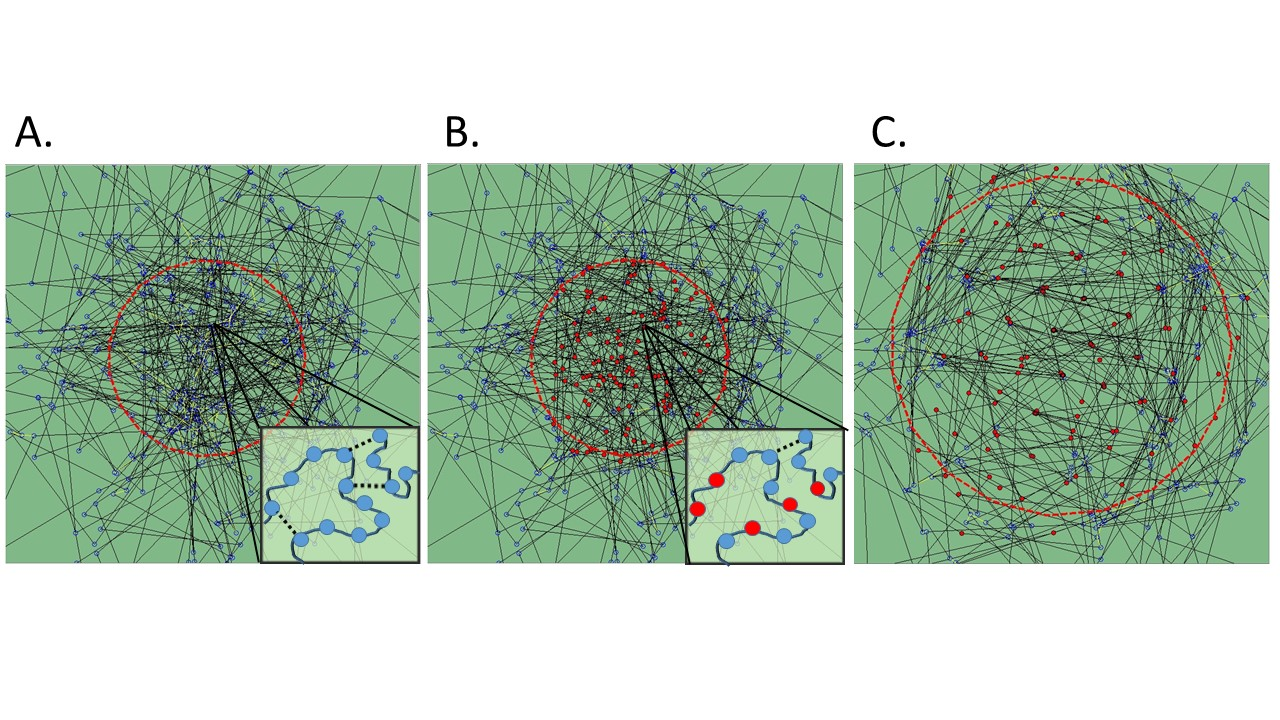
\includegraphics[width=0.9\linewidth, height=0.35\textheight]{threeStagesOfSimulation}
	\caption{\textbf{Stages in the Simulation of chromatin spatial organization post UV-C irradiation}. \textbf{A.} a Rouse chain of 500 monomers (circles) connected by harmonic spring (black lines) with a minimal length L0 is crossed-linked by harmonic springs (dashed lines in box) is simulated up to relaxation time, at which point a UV-C beam is vertically shot through a circular damage region (red dashed circle) around the polymer’s center-of-mass. \textbf{B.}  damaged monomers (red circles) are set to be distributed uniformly for each UV dose. Following UV-C irradiation, cross-links (dashed lines in box) to and from damaged monomers are removed. \textbf{C.} crowding of repair proteins is simulated by regions of exclusion centered around each damaged monomer. An elastic pushing force is applied to surrounding monomers with a maximal affect radius of rp. As a result, the damage region expands until reaching its maximal size 15 minutes post UV-C. The Region of Interest (ROI) is then determined as the circles containing 90\% of the damaged monomers (dashed red circle).}
	\label{fig:threeStagesOfSimulation}
	\end{figure}
	
	\subsection{Post repair stage}
	Fifteen minutes post UV-C we remove the exclusion region around damaged monomers. Cross-links are reintroduced by linking any two monomers located within an encounter distance of $\epsilon$ from one another. Cross-links post repair are allowed to be added up to the initial cross-linking percentage $\alpha$.
	
	\subsection{Measuring structural similarity}
	A measure of similarity between the polymer spatial organization before UV and post repair is based on the comparison of their encounter probability matrices. The polymer's encounter matrix just prior the onset of UV-irradiation is compared to that at end simulation time. The similarity values is given by the mean square error between matrices. 
			
	\bibliographystyle{plain}
	\bibliography{SimulationFrameworkForChromatineArchitecturePostUVC} % the bibliography.bib file 
\end{document}